% !TEX program = xelatex
\documentclass[aspectratio=169,12pt,fontset=none]{ctexbeamer}
\usetheme{Madrid}
\usecolortheme{whale}
\setbeamertemplate{navigation symbols}{}
\setbeamertemplate{footline}[frame number]

% 答辩演讲稿 — 共享导言（颜色、盒子、tikz、listings）
\usepackage{graphicx}
\usepackage{xcolor}
\usepackage{amsmath,amssymb}
\usepackage{booktabs}
\usepackage{longtable}
\usepackage{array}
\usepackage{multirow}
\makeatletter
\@ifclassloaded{beamer}{%
  % enumitem 与 beamer 的 enumerate 模板冲突，幻灯片侧不加载
}{%
  \usepackage{enumitem}%
}
\makeatother
\usepackage{hyperref}
\usepackage{listings}
\usepackage{tcolorbox}
\tcbuselibrary{breakable,skins,listings}
\usepackage{tikz}
\usetikzlibrary{positioning,fit,arrows.meta,calc,matrix,backgrounds,shapes.geometric}

\definecolor{PressRed}{RGB}{160,50,40}
\definecolor{AdaptGreen}{RGB}{30,110,60}
\definecolor{PruneOrange}{RGB}{180,90,20}
\definecolor{PosBlue}{RGB}{30,80,140}
\definecolor{CodeBg}{RGB}{248,248,252}
\definecolor{CodeFrame}{RGB}{200,200,210}
\definecolor{CodeKeyword}{RGB}{0,0,180}
\definecolor{CodeComment}{RGB}{100,100,100}
\definecolor{CodeString}{RGB}{163,21,21}

\newtcolorbox{philobox}[1][]{
  colback=blue!4!white, colframe=PosBlue, fonttitle=\bfseries,
  title={#1}, breakable, arc=2pt
}
\newtcolorbox{pressbox}[1][]{
  colback=red!4!white, colframe=PressRed, fonttitle=\bfseries,
  title={#1}, breakable, arc=2pt
}
\newtcolorbox{adaptbox}[1][]{
  colback=green!4!white, colframe=AdaptGreen, fonttitle=\bfseries,
  title={#1}, breakable, arc=2pt
}
\newtcolorbox{prunebox}[1][]{
  colback=orange!5!white, colframe=PruneOrange, fonttitle=\bfseries,
  title={#1}, breakable, arc=2pt
}

\tikzset{
  evt/.style={rectangle, rounded corners=2pt, draw=gray!60, fill=blue!5,
    align=left, minimum width=9cm, minimum height=0.75cm, font=\small},
  pres/.style={rectangle, draw=PressRed!70, fill=red!6, align=center,
    minimum width=2.4cm, minimum height=0.65cm, font=\footnotesize},
  comp/.style={rectangle, draw=PosBlue!70, fill=blue!6, align=center,
    minimum width=2.6cm, minimum height=0.7cm, font=\footnotesize},
  arrow/.style={-{Stealth[length=2mm]}, thick, draw=gray!60}
}

% 仓库根相对本目录：../../../
\newcommand{\repopath}[1]{\filepath{../../../#1}}

% Workbench GUI 字体（gui/public/fonts）
\newcommand{\ebguifontpath}{../../../gui/public/fonts/}

\makeatletter
\@ifclassloaded{beamer}{\usefonttheme{professionalfonts}}{}
\makeatother

\setmainfont{JetBrainsMonoNLNerdFont-Regular}[
  Path=\ebguifontpath,
  Extension=.ttf,
  BoldFont=JetBrainsMonoNLNerdFont-Bold,
  ItalicFont=JetBrainsMonoNLNerdFont-Italic,
  BoldItalicFont=JetBrainsMonoNLNerdFont-BoldItalic,
  Scale=0.92
]
\setmonofont{JetBrainsMonoNLNerdFont-Regular}[
  Path=\ebguifontpath,
  Extension=.ttf,
  BoldFont=JetBrainsMonoNLNerdFont-Bold,
  ItalicFont=JetBrainsMonoNLNerdFont-Italic,
  BoldItalicFont=JetBrainsMonoNLNerdFont-BoldItalic
]
\newfontfamily\ebproggy{ProggyCleanNerdFontMono-Regular}[
  Path=\ebguifontpath,
  Extension=.ttf
]

% 中文回退：Windows 用雅黑（与 GUI --font-ui 一致），WSL/TeX Live 用 Fandol
\IfFontExistsTF{Microsoft YaHei}{%
  \setCJKmainfont{Microsoft YaHei}[
    BoldFont={Microsoft YaHei Bold},
    ItalicFont={Microsoft YaHei},
    BoldItalicFont={Microsoft YaHei Bold}
  ]
  \setCJKsansfont{Microsoft YaHei}[
    BoldFont={Microsoft YaHei Bold}
  ]
}{%
  \setCJKmainfont{FandolSong-Regular}[
    Path=/usr/share/texlive/texmf-dist/fonts/opentype/public/fandol/,
    Extension=.otf,
    BoldFont={FandolSong-Bold},
    ItalicFont={FandolSong-Regular},
    BoldItalicFont={FandolSong-Bold}
  ]
  \setCJKsansfont{FandolHei-Regular}[
    Path=/usr/share/texlive/texmf-dist/fonts/opentype/public/fandol/,
    Extension=.otf,
    BoldFont={FandolHei-Bold}
  ]
}

\lstdefinestyle{ebbackupcpp}{
  language=C++,
  basicstyle=\ebproggy\footnotesize,
  keywordstyle=\color{CodeKeyword}\bfseries,
  commentstyle=\color{CodeComment}\itshape,
  stringstyle=\color{CodeString},
  numbers=left,
  numberstyle=\tiny\color{gray},
  stepnumber=1,
  numbersep=6pt,
  backgroundcolor=\color{CodeBg},
  frame=single,
  rulecolor=\color{CodeFrame},
  breaklines=true,
  showstringspaces=false,
  tabsize=2,
  captionpos=b
}
\lstdefinestyle{ebbackupjson}{
  basicstyle=\ebproggy\footnotesize,
  numbers=left,
  numberstyle=\tiny\color{gray},
  backgroundcolor=\color{CodeBg},
  frame=single,
  rulecolor=\color{CodeFrame},
  breaklines=true,
  tabsize=2
}
\lstdefinestyle{ebbackupts}{
  language=Java,
  basicstyle=\ebproggy\footnotesize,
  keywordstyle=\color{CodeKeyword}\bfseries,
  commentstyle=\color{CodeComment}\itshape,
  stringstyle=\color{CodeString},
  numbers=left,
  numberstyle=\tiny\color{gray},
  backgroundcolor=\color{CodeBg},
  frame=single,
  rulecolor=\color{CodeFrame},
  breaklines=true,
  tabsize=2
}

% 答辩演讲稿共享宏
\newcommand{\vtag}[1]{\texttt{v#1}}
\newcommand{\gitdesc}[1]{\texttt{#1}}
\newcommand{\filepath}[1]{\texttt{\small #1}}
\newcommand{\wave}[1]{\textbf{Wave #1}}

% 逐字稿：双时长标注
\newcommand{\timing}[2]{%
  \par\smallskip\noindent{\small\color{gray}%
    \textbf{口播时长}\quad 课程版：#1 \quad|\quad 技术版：#2}\par\smallskip}

% 口播正文
\newenvironment{say}{%
  \begin{tcolorbox}[colback=blue!3!white,colframe=PosBlue!60,arc=2pt,boxrule=0.4pt,left=4pt,right=4pt,top=3pt,bottom=3pt]
  \small
}{%
  \end{tcolorbox}
}

% 演示动作提示
\newcommand{\demo}[1]{%
  \par\noindent{\small\color{AdaptGreen!80!black}\textbf{[演示]}\ #1}\par}

% Beamer 幻灯片标题副标
\newcommand{\slidesubtitle}{ebbackup 数据备份软件 · \vtag{0.9.5}}

% 代码片段（\lstinputlisting 包装）
\newcommand{\codesnippet}[4]{%
  \lstinputlisting[style=#1,firstline=#2,lastline=#3]{../../../#4}}

\newcommand{\showcifloor}{%
  \codesnippet{ebbackupjson}{1}{13}{engine_cpp/bench/baselines/ci_floor.json}}

\newcommand{\showrepostats}{%
  \codesnippet{ebbackupcpp}{38}{59}{engine_cpp/src/store/repo_stats.cc}}

\newcommand{\showrunbackup}{%
  \codesnippet{ebbackupcpp}{764}{768}{engine_cpp/src/engine/backup_engine.cc}}

\newcommand{\showshim}{%
  \codesnippet{ebbackupcpp}{124}{134}{engine_cpp/workbench/ebbackup_workbench_shim.cc}}

\newcommand{\showpanelsurface}{%
  \codesnippet{ebbackupts}{141}{149}{gui/src/utils/themeSettings.ts}}


\title{ebbackup 数据备份软件}
\subtitle{\slidesubtitle\\《软件开发综合实验》答辩}
\author{recoveryProjects}
\date{2026-07-08 \quad commit \gitdesc{965431b}}

\begin{document}

%--- 1 封面 ---
\begin{frame}
  \titlepage
  \note{开场 30s：项目名称、课程、版本 v0.9.5 含 Workbench GUI。}
\end{frame}

%--- 2 定位 ---
\begin{frame}{一句话定位}
  \begin{philobox}[生态定位]
    不是「又一个 backup CLI」，而是在\textbf{可验证、可回归、可单机交付}前提下，把\textbf{内容寻址增量备份内核}做到本地吞吐与运维闭环足够强——用 \textbf{SI MB/s 数字}说话，而非形容词。
  \end{philobox}
  \vspace{0.4em}
  \begin{itemize}
    \item 内核即产品；不做云网盘、不做多租户
    \item 363 gtest + L1--L7 bench 硬门禁
    \item 可选桌面 Workbench（Tauri + Vue）
  \end{itemize}
  \note{强调与课程「数据备份软件」一致，但工程深度超出 baseline。}
\end{frame}

%--- 3 课程对照 ---
\begin{frame}{课程功能对照}
  % Beamer 精简：课程对照（半表）
\begin{table}
\centering
\tiny
\begin{tabular}{@{}ll@{}}
\toprule
课程项 & 实现 \\
\midrule
备份/还原 & 基础40 — \filepath{eb backup/restore} + GUI \\
特殊文件/元数据 & symlink + mtime/mode/uid \\
筛选/压缩/加密 & filter + LZ4/zstd + AES-GCM \\
GUI/定时/实时 & Workbench + schedule + watch \\
网络备份 & 刻意不做 \\
\bottomrule
\end{tabular}
\end{table}

  \note{完整表见逐字稿；网络备份主动说明生态边界。}
\end{frame}

%--- 4 架构与宪法 ---
\begin{frame}{内核架构}
  \resizebox{0.95\textwidth}{!}{%
    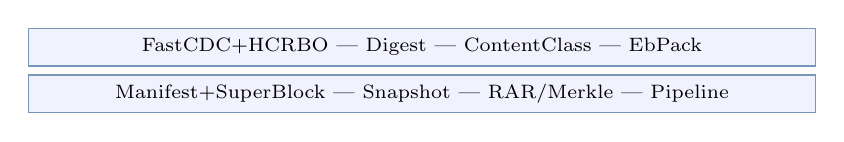
\begin{tikzpicture}[
      layer/.style={rectangle, draw=PosBlue!60, fill=blue!5, minimum width=10cm,
        minimum height=0.48cm, font=\scriptsize}
    ]
      \node[layer] (l1) {FastCDC+HCRBO | Digest | ContentClass | EbPack};
      \node[layer, below=0.1cm of l1] (l2) {Manifest+SuperBlock | Snapshot | RAR/Merkle | Pipeline};
    \end{tikzpicture}
  }
  \vspace{0.3em}
  \small 四条宪法：Content ID · 提交点 fsync · immutable floor · kAborted 可恢复
  \note{详细八层见逐字稿与 kernel-manual。}
\end{frame}

%--- 5 构件图 ---
\begin{frame}{构件图（物理体系结构）}
  % 物理构件图（课程「构件图」答辩口径）
\begin{figure}[htbp]
\centering
\begin{tikzpicture}[node distance=1.2cm and 1.4cm]
  \node[comp] (cli) {CLI\\\filepath{eb}};
  \node[comp, right=of cli] (dll) {SHARED DLL\\\filepath{ebbackup\_workbench}};
  \node[comp, right=of dll] (gui) {Workbench\\Tauri+Vue};
  \node[comp, below=1.4cm of dll] (core) {静态库\\\filepath{ebbackup\_core}};
  \draw[arrow] (cli) -- (core);
  \draw[arrow] (dll) -- (core);
  \draw[arrow] (gui) -- node[above,font=\tiny]{JSON shim} (dll);
  \node[below=0.3cm of core, font=\footnotesize, align=center] {ChunkStore / Pipeline / Manifest / Snapshot};
\end{tikzpicture}
\caption{构件依赖：GUI 不直连内核，经 JSON shim 调用 C API}
\label{fig:components}
\end{figure}

  \note{对应课程 UML 构件图要求；GUI 经 DLL JSON shim 解耦。}
\end{frame}

%--- 7 顺序图 ---
\begin{frame}{备份主路径}
  \resizebox{0.92\textwidth}{!}{%
    % 备份主路径顺序图（无 figure 外壳，供 Beamer resize）
\begin{tikzpicture}[node distance=0.55cm]
  \node[evt, minimum width=11cm, minimum height=0.55cm, font=\scriptsize] (u) {用户：\texttt{eb backup} 或 Workbench};
  \node[evt, below=of u, minimum width=11cm, minimum height=0.55cm, font=\scriptsize] (s) {Scan：遍历 + filter};
  \node[evt, below=of s, minimum width=11cm, minimum height=0.55cm, font=\scriptsize] (c) {Chunk：FastCDC + SHA256};
  \node[evt, below=of c, minimum width=11cm, minimum height=0.55cm, font=\scriptsize] (e) {Encode：LZ4/zstd + AES};
  \node[evt, below=of e, minimum width=11cm, minimum height=0.55cm, font=\scriptsize] (st) {Store：EbPack + chunk.idx};
  \node[evt, below=of st, minimum width=11cm, minimum height=0.55cm, font=\scriptsize] (m) {Commit：manifest + superblock};
  \draw[arrow] (u)--(s)--(c)--(e)--(st)--(m);
\end{tikzpicture}

  }
  \note{演示前可口述：scan$\rightarrow$chunk$\rightarrow$store$\rightarrow$manifest commit 提交点。}
\end{frame}

%--- 8 实测 ---
\begin{frame}{实测高光（L5/L7）}
  \begin{table}
    \centering\small
    \begin{tabular}{@{}lrr@{}}
    \toprule
    级别 & floor & 实测 \\
    \midrule
    L5 256MB & 105 & 170--172 MB/s \\
    L7 multi & 550 & 646--658 MB/s \\
    L3b ratio & 0.90 & 1.01--1.05 \\
    \bottomrule
    \end{tabular}
  \end{table}
  \note{完整表见逐字稿；数字来自 ci\_floor.json 与 CHANGELOG。}
\end{frame}

%--- 9 Wave5 ---
\begin{frame}{真实经历 I：Wave 5 正确性}
  \begin{pressbox}[P3 爆发 — \vtag{0.9.0}]
    Pipeline v4 多 worker 下 ChunkStore 全局锁导致 heap corruption（\texttt{0xC0000005}）与 \texttt{ForEachRecord} 重入死锁。L5 仍 $\sim$146 MB/s——若继续 chase 分数，生态因\textbf{不可恢复 crash} 归零。
  \end{pressbox}
  \vspace{0.3em}
  \textbf{决策}：16-shard 索引 + tombstone 锁序 + atomic finalize；\textbf{先修正确性再 Sprint}。
  \note{这是最有说服力的「工程取舍」故事。}
\end{frame}

%--- 10 Stage 3.2 ---
\begin{frame}{真实经历 II：Stage 3.2 剪枝}
  \begin{table}
    \centering\small
    \begin{tabular}{@{}lr@{}}
    \toprule
    Stage 3.2 L5 目标 & 280 MB/s \\
    v0.9.4 实测 & 171 MB/s（61\%） \\
    若 blocking & CI 100\% 红 \\
  \bottomrule
    \end{tabular}
  \end{table}
  \textbf{剪枝}：3.2 降为 aspirational nightly；3.1（105 MB/s）作 merge 门禁。
  \note{体现「测量立法」而非口号式目标。}
\end{frame}

%--- 11 Phase A ---
\begin{frame}{真实经历 III：CDC Phase A 止损}
  \begin{table}
    \centering\small
    \begin{tabular}{@{}lr@{}}
    \toprule
    Phase B（默认 stream） & 170--172 MB/s \\
    Phase A（\texttt{CDC\_FAST\_SLICE=1}） & $\sim$105 MB/s \\
    相对损失 & \textbf{-39\%} \\
  \bottomrule
    \end{tabular}
  \end{table}
  \textbf{结论}：实验路径 opt-in；immutable ratio 捕不到绝对 MB/s 劣化。
  \note{负向实验同样值得答辩讲述。}
\end{frame}

%--- 12 Workbench ---
\begin{frame}{Workbench 演示链}
  \begin{enumerate}
    \item 仓库：init / open（空仓库零统计，已修 manifest 路径）
    \item 备份：源路径校验 + 首次全量
    \item 快照：list / prune
    \item 恢复：\texttt{restore --at}
    \item GUI：透明度调节器、壁纸模式
  \end{enumerate}
  \vspace{0.3em}
  \small 详见 \filepath{docs/product/WORKBENCH\_GUI.md}
  \note{现场演示 3 分钟可录屏：创建仓库$\rightarrow$备份$\rightarrow$查看快照。}
\end{frame}

%--- 13 测试 ---
\begin{frame}{测试与门禁}
  \begin{itemize}
    \item \textbf{363} gtest + L1--L7 bench + powerfail + Rust IT
    \item immutable：reuse $\geq$90\%、ratio $\geq$0.90
    \item GitHub Actions：Windows + Linux
  \end{itemize}
  \note{ci\_floor.json 全文见逐字稿；强调机器可执行的完成定义。}
\end{frame}

%--- 14 理念对比 ---
\begin{frame}{开发理念 vs 课程软件工程}
  \resizebox{0.88\textwidth}{!}{%
    % 适应性工程环（无 figure 外壳，供 Beamer resize）
\begin{tikzpicture}[node distance=0.75cm]
  \node[evt, minimum height=0.55cm, font=\scriptsize] (b) {Bench/Profile 或 Bug（P1--P5）};
  \node[evt, below=of b, minimum height=0.55cm, font=\scriptsize] (h) {假设：改 X（不碰 Content ID）};
  \node[evt, below=of h, minimum height=0.55cm, font=\scriptsize] (i) {实现 + parity/powerfail};
  \node[evt, below=of i, minimum height=0.55cm, font=\scriptsize] (g) {ctest + bench\_check};
  \node[evt, below=of g, minimum height=0.55cm, font=\scriptsize] (d) {默认 / opt-in / CHANGELOG};
  \node[evt, below=of d, minimum height=0.55cm, font=\scriptsize] (p) {负向？剪枝回退};
  \draw[arrow] (b)--(h)--(i)--(g)--(d);
  \draw[arrow] (d)--(p);
  \draw[arrow] (p.west) -- ++(-1.0,0) |- (b.west);
\end{tikzpicture}

  }
  \vspace{0.2em}
  \footnotesize
  \textbf{相同}：迭代、分层、测试、文档沉淀 \quad
  \textbf{不同}：测量驱动 vs 纸面需求锁定
  \note{坦诚：StarUML 四图需从事后文档导出补交课程格式。}
\end{frame}

%--- 15 真实产品化 ---
\begin{frame}{产品化实验（GUI）}
  \textbf{空仓库}：\texttt{repo\_info} 曾报 manifest 缺失 $\rightarrow$ \texttt{ComputeRepoStats} 修复\\
  \textbf{透明度}：WebView2 嵌套 \texttt{color-mix} 失效 $\rightarrow$ 预计算 \texttt{rgba} alpha\\
  \textbf{备份 UX}：\texttt{source path not found} $\rightarrow$ 路径存在性校验
  \note{来自真实联调，非编造。}
\end{frame}

%--- 15b 可证明备份 ---
\begin{frame}{可证明备份（Wave A--M）}
  \begin{itemize}
    \item \textbf{路径索引}：\texttt{path\_index.jsonl} + 分页 \texttt{browse-page}（ABI v14）
    \item \textbf{Merkle Diff}：\texttt{added/modified} 附 \texttt{merkle\_proof}（v15）
    \item \textbf{恢复验收}：\texttt{export\_restore\_report} + GUI「验收报告」
    \item \textbf{三路就地}：base/target/live + \texttt{both\_changed}（Wave M, v23）
    \item \textbf{Win 元数据}：Manifest v5 + ADS/hardlink/junction（Wave B/E, v16）
  \end{itemize}
\end{frame}

%--- 15c 能力 Wave 弧 ---
\begin{frame}{能力 Wave 弧（N$\rightarrow$T）}
  \small
  \begin{tabular}{@{}llp{7.5cm}@{}}
  \toprule
  Wave & ABI & 交付 \\
  \midrule
  N--O+ & v24--26 & 可达性、RPO、服务化、多 Profile \\
  P--Q & v27 & SQLite/Registry/VHDX 插件 \\
  R & v28 & 智能排除建议 + GUI 采纳 \\
  T & v29 & 备份窗口 + deadline 降级 \\
  \bottomrule
  \end{tabular}
  \vspace{0.4em}\\
  \footnotesize 归档：\filepath{docs/WAVE\_ARCHIVE.md} · 363 gtest 全绿
\end{frame}

%--- 16 总结 ---
\begin{frame}{总结}
  \begin{enumerate}
    \item \textbf{功能}：课程基础 + 多项扩展（无网络）
    \item \textbf{工程}：宪法 + bench 门禁 + 363 测试 + ABI v29
    \item \textbf{经历}：Wave5 正确性 / 3.2 剪枝 / Phase A 止损 / Wave A--T 能力弧
    \item \textbf{交付}：CLI + DLL + Workbench + CMake + CI
  \end{enumerate}
  \vspace{0.5em}
  \centering\Large 谢谢 · Q\&A
  \note{预留问答：EbPack、Qt vs Tauri、与 restic 差异、immutable floor。}
\end{frame}

\end{document}
